%iffalse
\let\negmedspace\undefined
\let\negthickspace\undefined
\documentclass[journal,12pt,onecolumn]{IEEEtran}
\usepackage{cite}
\usepackage{amsmath,amssymb,amsfonts,amsthm}
\usepackage{algorithmic}
\usepackage{graphicx}
\usepackage{textcomp}
\usepackage{xcolor}
\usepackage{txfonts}
\usepackage{listings}
\usepackage{enumitem}
\usepackage{mathtools}
\usepackage{pgfplots}
\usepackage{gensymb}
\usepackage{tikz}
\usetikzlibrary{patterns}
\usepackage{comment}
\usepackage[breaklinks=true]{hyperref}
\usepackage{tkz-euclide} 
\usepackage{listings}
\usepackage{gvv}                                        
%\def\inputGnumericTable{}                                 
\usepackage[latin1]{inputenc}                                
\usepackage{color}          
\usepackage{circuitikz}
\usepackage{array}                                            
\usepackage{longtable}                                       
\usepackage{calc}                                             
\usepackage{multirow}                                         
\usepackage{hhline}                                           
\usepackage{ifthen}                                           
\usepackage{lscape}
\usepackage{tabularx}
\usepackage{array}
\usepackage{float}

\usepackage{enumitem}
\usepackage{xcolor}
%\usepackage{multicol}


\newtheorem{theorem}{Theorem}[section]
\newtheorem{problem}{Problem}
\newtheorem{proposition}{Proposition}[section]
\newtheorem{lemma}{Lemma}[section]
\newtheorem{corollary}[theorem]{Corollary}
\newtheorem{example}{Example}[section]
\newtheorem{definition}[problem]{Definition}
\newcommand{\BEQA}{\begin{eqnarray}}
\newcommand{\EEQA}{\end{eqnarray}}
\newcommand{\define}{\stackrel{\triangle}{=}}
\theoremstyle{remark}
\newtheorem{rem}{Remark}

\title{2023-ME-53-65}
\author{AI24BTECH11023 - Tarun Reddy Pakala}
\begin{document}
\bibliographystyle{IEEEtran}

\maketitle
\bigskip
\renewcommand{\thefigure}{\theenumi}
\renewcommand{\thetable}{\theenumi}
\begin{enumerate}[start=53]
\item A part, produced in high volumes, is dimensional as shown. The machining process making this part is known to be statistically in control based on sampling data. The sampling data shows that $D_1$ follows a normal distribution with a mean of $20\;mm$ and a standard deviation of $0.3\;mm$, while $D_2$ follows a normal distribution with a mean of $35\;mm$ and a standard deviation of $0.4\;mm$. An inspection of dimension $C$ is carried out in a sufficiently large number of parts.\\ To be considered under six-sigma process control, the upper limit of dimension $C$ should be \underline{\hspace{2cm}} $mm$.\\ \brak{Rounded\;off\;to\;one\;decimal\;place}
%input for figure 1
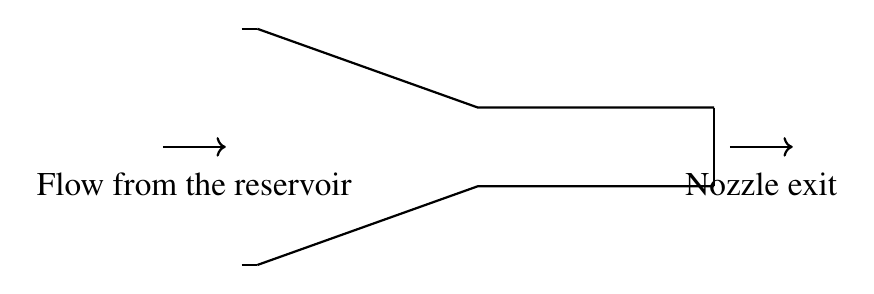
\begin{tikzpicture}
    % Draw the nozzle shape with short vertical lines at the opening
    \draw[thick] (-3,1.5) -- (-2.8,1.5);
    \draw[thick] (-3,-1.5) -- (-2.8,-1.5);
    \draw[thick] (-2.8,1.5) -- (0,0.5) -- (3,0.5);
    \draw[thick] (-2.8,-1.5) -- (0,-0.5) -- (3,-0.5);
    
    % Vertical line at the nozzle exit
    \draw[thick] (3,0.5) -- (3,-0.5);

    % Flow direction arrows
    \draw[->, thick] (-4,0) -- (-3.2,0);
    \draw[->, thick] (3.2,0) -- (4,0);

    % Labels for the flow and nozzle exit, placed below arrows
    \node[below] at (-3.6,-0.2) {\large Flow from the reservoir};
    \node[below] at (3.6,-0.2) {\large Nozzle exit};
\end{tikzpicture}

\item A coordinate measuring machine \brak{\text{CMM}} is used to determine the distance between Surface SP and Surface SQ of an approximately cuboidal shaped part. Surface SP is declared as the datum as per the engineering drawing used for manufacturing this part. The CMM is used to measure four points $P_1,\;P_2,\;P_3,\;P_4$ on surface $SP$, and four points $Q_1,\;Q_2,\;Q_3,\;Q_4$ on Surface $SQ$ as shown. A regression procedure is used to fit the necessary planes.\\ The distance between the two fitted planes is 
\underline{\hspace{2cm}} $mm$.\\ \brak{Answer\;in\;integer}
%input for figure 2
\begin{figure}[!ht]
\centering
\resizebox{3cm}{3cm}{%
\begin{circuitikz}
\tikzstyle{every node}=[font=\LARGE]
\draw [ line width=0.6pt](2.75,12) to[sinusoidal voltage source, sources/symbol/rotate=auto] (3.25,11.5);
\draw [ line width=0.6pt](3.25,11.75) to[european resistor] (9.5,11.75);
\draw [line width=0.6pt, ->, >=Stealth] (9.5,11.75) -- (9.5,11);
\draw [ line width=0.6pt](4,12.25) to[short] (4,11.25);
\draw [ line width=0.6pt](4,11.5) to[short] (4,11);
\draw [ line width=0.6pt](8.75,12.25) to[short] (8.75,11);
\draw [ line width=0.6pt](4,11.25) to[short] (4.5,11.25);
\draw [ line width=0.6pt](8.75,11.25) to[short] (8.25,11.25);
\draw [ line width=0.6pt](4.25,11.25) to[short] (5.25,11.25);
\draw [ line width=0.6pt](8.25,11.25) to[short] (7.25,11.25);
\draw [ line width=0.6pt](5,11.25) to[european resistor] (5,8.5);
\draw [ line width=0.6pt](7.5,11.25) to[european resistor] (7.5,8.5);
\draw [ line width=0.6pt](4.75,8.5) to[short] (8,8.5);
\draw [line width=0.6pt, ->, >=Stealth] (6.25,8.5) -- (6.25,7.75);
\node [font=\normalsize] at (6.75,8) {Bus 3};
\node [font=\normalsize] at (4,12.5) {Bus 1};
\node [font=\normalsize] at (8.75,12.5) {Bus 2};
\node [font=\normalsize] at (6.25,12.25) {j q};
\node [font=\normalsize] at (4.5,10) {j r};
\node [font=\normalsize] at (8.25,9.75) {j p};
\end{circuitikz}
}%

\label{fig:my_label}
\end{figure}

\item A solid part \brak{\text{see figure}} of polymer material is to be fabricated by additive manufacturing \brak{\text{AM}} in square-shaped layers starting from the bottom of the part working upwards. The nozzle diameter of the AM machine is $\frac{a}{10}\;mm$ and the nozzle follows a linear serpentine path parallel to the sides of the square layers with a feed rate of $\frac{a}{5}\;\frac{mm}{min}$.\\ Ignore any tool path motions other than those involved in adding material, and any other delays between layers or the serpentine scan lines.\\ The time taken to fabricate this part is \underline{\hspace{2cm}} minutes.\\ \brak{Answer\;in\;integer}
%input for figure 3
\begin{figure}[!ht]
\centering
\resizebox{3cm}{3cm}{%
\begin{circuitikz}
\tikzstyle{every node}=[font=\small]
\draw (4.25,12.25) to[battery1] (4.25,7.75);
\draw (4.25,12.25) to[short] (6.25,12.25);
\draw (4.25,7.75) to[short] (6.25,7.75);
\draw (6.25,12.25) to[R] (6.25,10.25);
\draw (6.25,10.25) to[R] (6.25,7.75);
\draw (6.25,10.25) to[short] (8.75,10.25);
\draw (6.25,7.75) to[short] (8.75,7.75);
\draw (8.75,7.75) to[R] (8.75,9.25);
\draw (8.75,10.25) to[D] (8.75,9);
\node [font=\small] at (4,10.25) {+};
\node [font=\small] at (4,9.75) {-};
\node [font=\small] at (4.75,10.5) {24 Volt};
\node [font=\small] at (6.75,11.25) {12 k$\Omega$};
\node [font=\small] at (6.75,9) {6 k$\Omega$};
\node [font=\small] at (8,8.5) {3.3 k$\Omega$};
\end{circuitikz}
}%

\label{fig:my_label}
\end{figure}

\item An optical flat is used to measure the height difference between a reference slip gauge $A$ and a slip gauge $B$. Upon viewing via the optical flat using a monochromatic light of wavelength $0.5\;\mu m,\;12$ fringes were observed over a length of $15\;mm$ of gauge $B$. If the gauges are placed $45\;mm$ apart, the height difference of the gauge is \underline{\hspace{2cm}}. $\mu m$.\\ \brak{Answer\;in\;integer} 
%input for figure 4
\begin{figure}[H]
\centering
\resizebox{3cm}{3cm}{%
\begin{circuitikz}
\tikzstyle{every node}=[font=\small]
\draw [->, >=Stealth] (3.5,10.75) -- (3.5,13.75);
\draw [->, >=Stealth] (3.5,10.75) -- (10.75,10.75);
\draw [->, >=Stealth] (2.25,10.75) -- (3.25,10.75);
\draw [dashed] (4.5,13.25) -- (4.5,8.25);
\draw [dashed] (7.25,13.25) -- (7.25,8.25);
\draw [dashed] (10,13.25) -- (10,8.25);
\draw [dashed] (2,8.25) -- (10,8.25);
\draw [dashed] (2,13) -- (10,13);
\draw [short] (4.5,10.75) -- (7.25,11.75);
\draw [short] (7.25,11.75) -- (10,9.75);
\draw [short] (4.5,10.75) -- (10,9.75);
\node [font=\small] at (2.5,11) {$M>1$};
\node [font=\small] at (3.5,14) {$y$};
\node [font=\small] at (11,10.75) {$x$};
\node [font=\small] at (4.5,8) {$X_A$};
\node [font=\small] at (7.25,8) {$X_B$};
\node [font=\small] at (10,8) {$X_C$};
\node [font=\small] at (1.75,8.25) {$Y_{II}$};
\node [font=\small] at (1.75,13) {$Y_I$};
\node [font=\small] at (5.5,11) {$\alpha$};
\node [font=\small] at (6.5,10.5) {$\alpha$};
\node [font=\small] at (9,10) {$2\alpha$};
\end{circuitikz}
}%
\label{fig:my_label}
\end{figure}

\item Ignoring the small elastic region, the true stress $\brak{\sigma}$- true strain $\brak{\epsilon}$ variation of a material beyond yielding follows the equation $\sigma=400\epsilon^{0.3}\;MPa$. The engineering ultimate tensile strength value of this material is \underline{\hspace{2cm}} $MPa$.\\ \brak{Rounded\;off\;to\;one\;decimal\;place}
\item The area moment of inertia about $y$-axis of a linearly tapered section shown in the figure is \underline{\hspace{2cm}} $m^4$.\\ \brak{Answer\;in\;integer}
%input for figure 5
\begin{figure}[!ht]
\centering
\resizebox{3cm}{3cm}{%
\begin{circuitikz}
\tikzstyle{every node}=[font=\small]
\draw [line width=0.6pt, short] (4,10.75) -- (8.25,10.75);
\draw [line width=0.6pt, short] (8.25,10.75) -- (9.75,12);
\draw [line width=0.6pt, short] (8.25,10.25) -- (9.75,11.5);
\draw [line width=0.6pt, short] (8.25,10.25) -- (9.75,9.25);
\draw [line width=0.6pt, short] (4,9.75) -- (8.25,9.75);
\draw [line width=0.6pt, ->, >=Stealth] (9.75,11.75) -- (10.25,12.25);
\draw [line width=0.6pt, ->, >=Stealth] (9.5,9) -- (10,8.5);
\draw [line width=0.6pt, ->, >=Stealth] (3.75,10.25) -- (5,10.25);
\node [font=\small] at (3.5,10.25) {$Q$};
\node [font=\small] at (10.5,12.5) {$Q_1$};
\node [font=\small] at (10.25,8.25) {$Q_2$};
\draw [line width=0.6pt, short] (8.25,9.75) -- (9.25,9);
\end{circuitikz}
}%

\end{figure}

\item A cylindrical bar has a length $L=5\;m$ and cross section are $S=10\;m^2$. The bar is made of a linear elastic material with a density $\rho =2700\frac{kg}{m^3}$ and Young's modulus $E=70\;GPa$. The bar is suspended as shown in the figure and is in a state of uniaxial tension due to its self-weight.\\ The elastic strain energy stored in the bars equals \underline{\hspace{2cm}} $J$.\brak{Rounded\;off\;to\;two\;decimal\;places}\\ Take the acceleration due to gravity as $g=9.8\;\frac{m}{s^2}$.
%input for figure 6
\begin{figure}[H]
\centering
\resizebox{3cm}{3cm}{%
\begin{circuitikz}
\tikzstyle{every node}=[font=\large]
\draw [ line width=0.6pt ] (5.5,12.5) rectangle (7.5,6.25);
\draw [line width=0.6pt, dashed] (6.5,12.5) -- (6.5,6.25);
\draw [line width=0.6pt, dashed] (4.75,12.5) -- (8.5,12.5);
\draw [line width=0.6pt, dashed] (4.75,12.75) -- (8.5,12.75);
\draw [line width=0.6pt, dashed] (4.75,13) -- (8.5,13);
\draw [line width=0.6pt, dashed] (4.75,13.25) -- (8.5,13.25);
\draw [line width=0.6pt, dashed] (4.75,13.5) -- (8.5,13.5);
\draw [line width=0.6pt, ->, >=Stealth] (4.5,10.5) -- (4.5,8.75);
\draw [line width=0.6pt, <->, >=Stealth] (8.5,12.5) -- (8.5,6.25);
\node [font=\large] at (4,9.75) {$g$};
\node [font=\large] at (9.25,9.5) {L};
\end{circuitikz}
}%

\label{fig:my_label}
\end{figure}

\item A cylinder transmission shaft of length $1.5\;m$ and diameter $100\;mm$ is made of a linear elastic material with a shear modulus $80\;GPa$. While operating at $500\;rpm$, the angle of twist across its length is found to be $0.5$ degrees.\\\\ The power transmitted by the shaft at this speed is \underline{\hspace{2cm}} $kW$. \brak{Rounded\;off\;to\;two\;decimal\;places}\\ Take $\pi =3.14$. 
\item Consider a mixture of two ideal gases, $X$ and $Y$, with molar masses $\Bar{M_X}=10\;\frac{kg}{kmol}$ and $\Bar{M_Y}=20\;\frac{kg}{kmol}$, respectively, in a container. The total pressure in the container is $100\;kPa$, the total volume if the container is $10\;m^3$ and the temperature of the contents of the container is $300\;K$. If the mass of gas-$X$ in the container is $2\;kg$, then the mass of the gas-$Y$ in the container is \underline{\hspace{2cm}}$kg$.\brak{Rounded\;off\;to\;one\;decimal\;place}\\ Assume that the universal gas constant is $8314\;J\;kmol^{-1}K^{-1}$.
\item The velocity field of a certain two-dimensional flow is given by $$\textbf{V}\brak{x,y}=k\brak{x\hat{i}-y\hat{j}}$$ where $k=2\;s^{-1}$. The coordinates $x$ and $y$ are in meters. Assume gravitational effects to be negligible.\\If the density of the fluid is $1000\frac{kg}{m^3}$ and the pressure at the origin is $100\;kPa$, the pressure at the location \brak{2\;m,\;2\;m} is \underline{\hspace{2cm}} $kPa$.\\ \brak{Answer\;in\;integer}
\item Consider a unidirectional fluid flow with the velocity field given by $$\textbf{V}\brak{x,y,z,t}=u\brak{x,t}\;\hat{i}$$ where $u\brak{0,t}=1$. If the spatially homogeneous density field varies with time $t$ as $$\rho\brak{t}=1+0.2e^{-t}$$ the value of $u\brak{2,1}$ is \underline{\hspace{2cm}}.\brak{Rounded\; off \;to\; two\; decimal\; places}\\ Assume all quantities to be dimensionless. 
\item The figure shows two fluids held by a hinged gate. The atmospheric pressure is $P_a=100\;kPa$. The moment per unit width about the base of the hing is \underline{\hspace{2cm}} $\frac{kNm}{m}$.\brak{Rounded\;off\;to\;one\;decimal\;place}\\ Take the acceleration due to gravity to be $g=9.8\frac{m}{s^2}$.
%input for figure 7
\begin{figure}[H]
\centering
\resizebox{3cm}{3cm}{%
\begin{circuitikz}
\tikzstyle{every node}=[font=\small]
\draw [line width=1.4pt, short] (8,13) -- (8,7.25);
\draw [line width=0.6pt, short] (3,7.25) -- (10.5,7.25);
\draw [line width=0.6pt, short] (3,7.25) -- (3,13);
\draw [line width=0.6pt, short] (3,12.75) -- (8,12.75);
\draw [line width=0.6pt, short] (3,10.75) -- (8,10.75);
\draw [line width=0.6pt, <->, >=Stealth] (3.75,12.75) -- (3.75,10.75);
\draw [line width=0.6pt, <->, >=Stealth] (3.75,10.75) -- (3.75,7.25);
\draw [line width=0.6pt, ->, >=Stealth] (8.75,11.75) -- (8.75,10.75);
\node [font=\small] at (3.25,11.75) {$1\; m$};
\node [font=\small] at (3.25,9) {$2\;m$};
\node [font=\small] at (5.5,11.75) {$1000\; \frac{kg}{m^3}$};
\node [font=\small] at (5.5,9) {$2000 \;\frac{kg}{m^3}$};
\node [font=\small] at (6,6.5) {Not to scale};
\node [font=\small] at (9,11.25) {$g$};
\node [font=\small] at (9,13) {$P_a$};
\node [font=\small] at (5.25,13.25) {$P_a$};
\node [font=\Huge] at (8,7.5) {.};
\draw [line width=0.6pt, ->, >=Stealth] (8.25,7.5) -- (8.75,8);
\node [font=\small] at (9.25,8.25) {Hinge};
\end{circuitikz}
}%

\label{fig:my_label}
\end{figure}

\item An explosion at time $t=0$ releases energy $E$ at the origin in a space filled with a gas of density $\rho$. Subsequently, a hemispherical blast wave propagates radially outwards as shown in the figure.\\ Let $R$ denote the radius of the hemisphere blast wave. The radius $R$ follows the relationship $R=kt^aE^b\rho^c$, where $k$ is a dimensionless constant. The value of exponent $a$ is \underline{\hspace{2cm}}.\\ \brak{Rounded\;off\;to\;one\;decimal\;place}\\
%input for figure 8
    \begin{figure}[H]
\raggedright
\resizebox{3cm}{3cm}{%
\begin{circuitikz}
\tikzstyle{every node}=[font=\small]
\draw [->, >=Stealth] (0.5,8) -- (0.5,12.5);
\draw [->, >=Stealth] (0.5,8) -- (6.5,8);
\draw [->, >=Stealth] (7,8) -- (13.25,8);
\draw [->, >=Stealth] (7,8) -- (7,12.5);
\draw [dashed] (1,12) -- (1,8.5);
\draw [dashed] (3,12) -- (3,8.75);
\draw [dashed] (5,12) -- (5,8.5);
\draw [short] (0.5,9.5) -- (1,9.5);
\draw [short] (1,9.5) -- (1,11.5);
\draw [short] (1,11.5) -- (3.5,11.5);
\draw [short] (3.5,11.5) -- (4.25,9.25);
\draw [short] (4.25,9.25) -- (5,9.25);
\draw [dashed] (7.5,12.25) -- (7.5,8.75);
\draw [dashed] (9.5,12.25) -- (9.5,8.75);
\draw [dashed] (12,12.25) -- (12,9);
\node [font=\small] at (8.5,12) {$Y_{II}$};
\node [font=\small] at (7.5,8.5) {$X_A$};
\node [font=\small] at (9.5,8.5) {$X_B$};
\node [font=\small] at (12,8.75) {$X_C$};
\node [font=\small] at (1,8.25) {$X_A$};
\node [font=\small] at (3,8.5) {$X_B$};
\node [font=\small] at (5,8.5) {$X_C$};
\node [font=\small] at (6.5,11.25) {P};
\node [font=\small] at (0.25,11.5) {P};
\node [font=\small] at (4,7.75) {$x$};
\node [font=\small] at (10.5,7.75) {$x$};
\node [font=\small] at (1.75,11.75) {$Y_I$};
\draw [short] (7,9.5) -- (8,9.5);
\draw [short] (8,9.5) -- (8,11.75);
\draw [short] (8,11.75) -- (12,11.75);
\end{circuitikz}
}%

\end{figure}

\end{enumerate}
\end{document}
